\documentclass{standalone}
% font set
\usepackage{ctex}
\usepackage{fontspec}
\usepackage[T1]{fontenc}
\usepackage[sc]{mathpazo}
\usepackage{anyfontsize}
\setmainfont{Source Serif 4}
\setsansfont{Source Sans 3}
\setmonofont{Menlo}
\setCJKmainfont[BoldFont=黑体-简 中等,ItalicFont=楷体-简 常规体]{宋体-简 常规体}

% colors
\usepackage[dvipsnames]{xcolor}
\definecolor{pku-red}{RGB}{139,0,18}
\usepackage{colortbl}
\newcommand{\light}[1]{\textcolor{Orchid}{#1}}
\newcommand{\contrastlight}[1]{\textcolor{TealBlue}{#1}}

% plots
\usepackage{tikz}
\usepackage{tikz-cd}
\usetikzlibrary{arrows}
\usetikzlibrary{arrows.meta,positioning,calc,3d}
\usepackage{pgfplots}
\pgfplotsset{compat=newest}
\tikzset{
    punkt/.style={
        rectangle,
        rounded corners,
        draw=black, very thick,
        minimum height=2em,
        inner sep=6pt,
        text centered,
        fill=gray!30
    }
}

% math package
\let\Bbbk\relax
\usepackage{amsmath}
\usepackage{mathrsfs}
\usepackage{amssymb}
\usepackage{amsfonts}
\usepackage{stmaryrd}
\usepackage{latexsym}
\usepackage{extarrows}
\SetSymbolFont{stmry}{bold}{U}{stmry}{m}{n}

\begin{document}
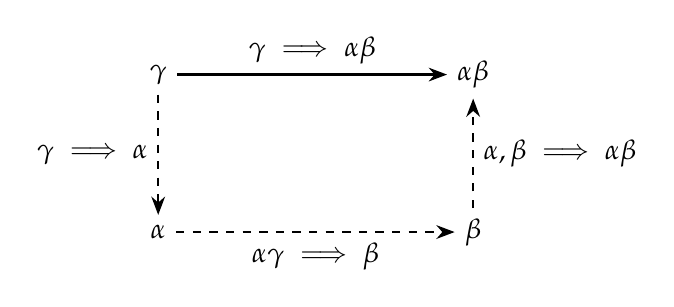
\begin{tikzpicture}[thick]
    \node (gamma) at (0,0) {$\gamma$};
    \node (ab) at (4,0) {$\alpha\beta$};
    \node (a) at (0,-2) {$\alpha$};
    \node (b) at (4,-2) {$\beta$};
    \draw[-Stealth] (gamma) -- node[above] {$\gamma\implies\alpha\beta$} (ab);
    \draw[-Stealth,dashed] (gamma) -- node[left] {$\gamma\implies\alpha$} (a);
    \draw[-Stealth,dashed] (a) -- node[below] {$\alpha\gamma\implies\beta$} (b);
    \draw[-Stealth,dashed] (b) -- node[right] {$\alpha,\beta\implies\alpha\beta$} (ab);
\end{tikzpicture}
\end{document}